%==========================================================================
%  TRES0312 Fysikk — Foiler-mal
%
%  MØrk/lys modus: kommenter ut én av de to linjene nedenfor.
%==========================================================================
\newif\ifdarkmode
\darkmodetrue      % ← mørk modus
%\darkmodefalse   % ← lys modus  (fjern % foran og legg % foran linjen over)

\documentclass[aspectratio=169, 12pt]{beamer}

\usepackage{amd-beamer}
\usetikzlibrary{overlay-beamer-styles}
\usetikzlibrary{calc}

%--------------------------------------------------------------------------
%  DOKUMENTINFO
%--------------------------------------------------------------------------
\title{Dynamikk}
\subtitle{TRES0312 --- Krefter i planet: dekomponering og skråplan}
\author{Ben David Normann}
\date{\today}

%--------------------------------------------------------------------------
%  SEKSJONSKONTEKST
%--------------------------------------------------------------------------
\setcounter{section}{4}   % Kapittel 4: "Dynamikk"

\begin{document}

%--------------------------------------------------------------------------
%  SLIDE 1 — TITTELSIDE
%--------------------------------------------------------------------------
\begin{frame}[plain]
  \titlepage
  \dekkerdelkap{kapittel 4.4--4.4.1}
\end{frame}

%--------------------------------------------------------------------------
%  SLIDE 2 — Tre kjappe fra forrige gang (krefter i dagliglivet)
%--------------------------------------------------------------------------
\begin{frame}{}

  \repetisjon{Tre kjappe fra forrige gang}{%
    \begin{enumerate}[1.]
      \item Skriv opp Hookes lov. Hva betyr minustegnet?
      \item Hva er sammenhengen mellom normalkraft $N$, friksjonskraft $R$ og underlagskraft $\vec{U}$?
      \item Hva er forskjellen mellom statisk og kinetisk friksjonskoeffisient, $\mu_s$ og $\mu_k$?
    \end{enumerate}
  }

\end{frame}

%--------------------------------------------------------------------------
%  SLIDE 3 — Oppsummering: Dekomponering av Newtons lover
%--------------------------------------------------------------------------
\begin{frame}{}

  \oppsum{Dekomponering av Newtons lover}{%
  Når vi løser oppgaver med krefter i planet, er det viktig å innføre et koordinatsystem, og deretter dekomponere Newtons lover. Med koordinater $x$ og $y$ i planet:
  \[
    \sum\vec{F} = m\vec{a}\quad\Longrightarrow\quad
    \begin{cases}
      \sum F_x = ma_x\\[4pt]
      \sum F_y = ma_y
    \end{cases}
  \]
  Helt tilsvarende for Newtons første lov, eller andre lover på vektorform.
  }

\end{frame}

%--------------------------------------------------------------------------
%  SLIDE 4 — Oppsummering: Algoritme
%--------------------------------------------------------------------------
\begin{frame}{}

  \oppsum{Algoritme for løsing av sammensatte kraftoppgaver}{%
  \begin{enumerate}[1.]
    \item Tegn figur av problemet, med relevante krefter.
    \item Skriv ned de relevante lovene.
    \item Gjør et hensiktsmessig valg av koordinatsystem.
    \item Dekomponer vektorlovene i koordinatsystemet.
    \item Løs settet med skalare likninger for de ukjente.
  \end{enumerate}
  }

\end{frame}

%--------------------------------------------------------------------------
%  SLIDE 5 — Eksempel: Slede i skråplan holdt av fjær
%--------------------------------------------------------------------------
\begin{frame}{Eksempel: algoritmen i bruk}

  \exmat{4.9}{Slede i skråplan holdt av fjær}{%
  En slede med Dashman, samlet masse $m$, ligger i ro på et friksjonsfritt skråplan med helningsvinkel $\theta = 30^\circ$. Sleden er festet til en fjær med fjærkonstant $k = 180\,\mathrm{N/m}$, strukket $x = 12\,\mathrm{cm}$ fra likevekt.
  \begin{enumerate}[a)]
    \item Tegn inn kreftene som virker på sleden.
    \item Regn ut fjærkrafta $F_k$.
    \item Finn massen $m$ til sleden.
  \end{enumerate}
  }

\end{frame}

%--------------------------------------------------------------------------
%  SLIDE 6 — Figur + løsning: krefter på sleden
%--------------------------------------------------------------------------
\begin{frame}{}

  \begin{columns}[T]
    \begin{column}{0.46\textwidth}
      \centering
      \begin{tikzpicture}
        \node[anchor=south west, inner sep=0] (image) at (0,0) {%
          \ifdarkmode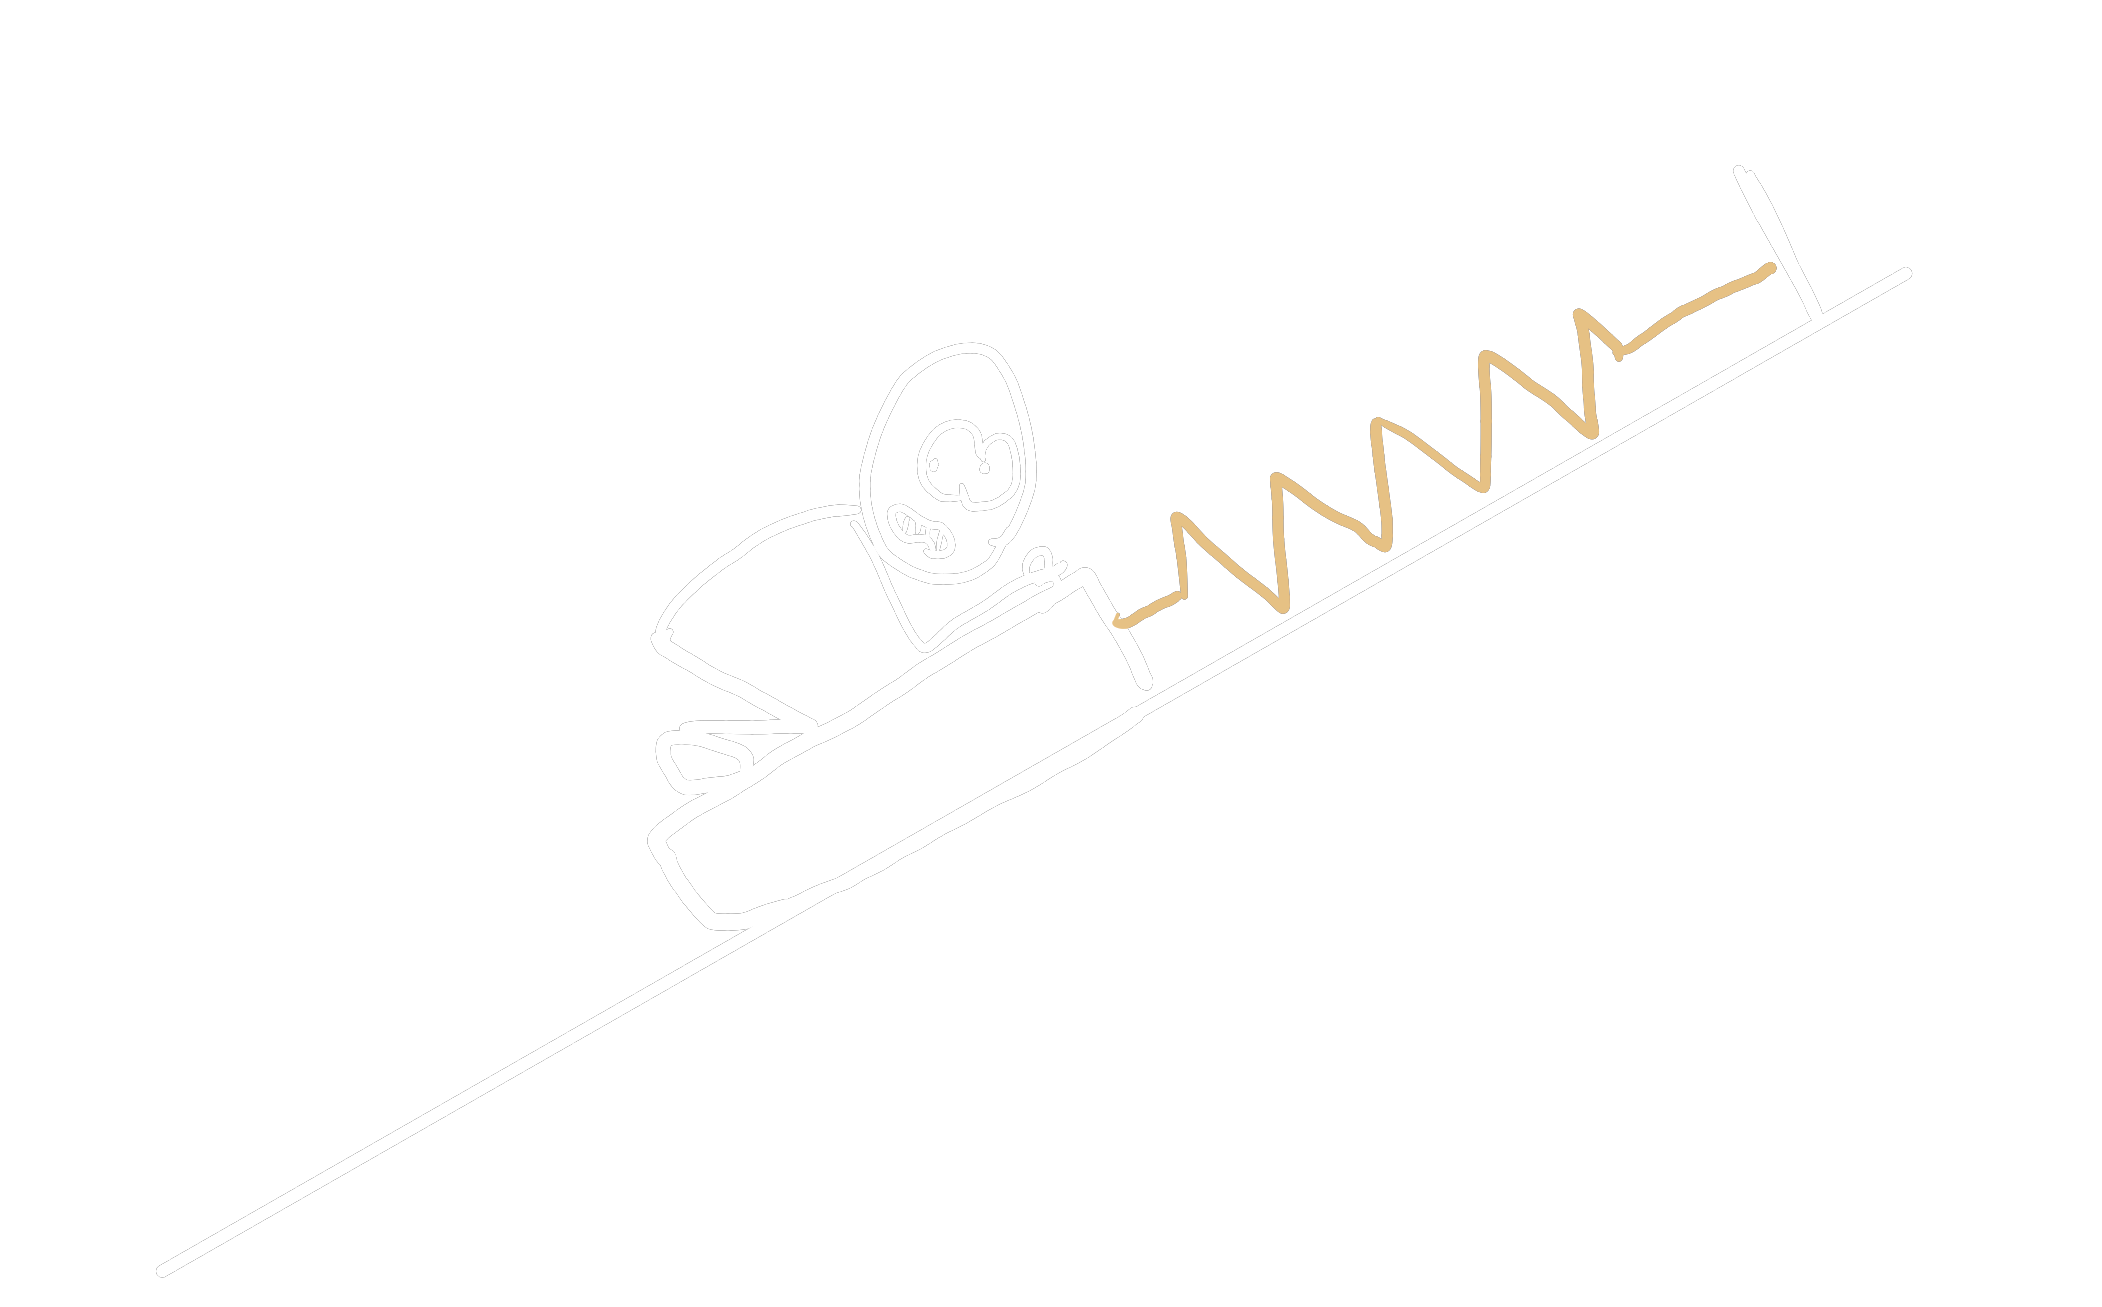
\includegraphics[width=5.6cm]{Images/Dashman_slede_fjaer_skraplan_mork.png}\else
\includegraphics[width=5.6cm]{Kapittel4:Dynamikk/Dashman_slede_fjaer_skraplan.png}\fi%
        };
        \begin{scope}[x={(image.south east)}, y={(image.north west)}]
          \draw[-{Stealth[length=9pt,width=6pt]}, line width=2pt, defscol]
            (0.419,0.357) -- (0.3481,0.5562);
          \node[left=2pt, defscol, font=\scriptsize\bfseries] at (0.3481,0.5562) {$\vec{N}$};
          \draw[-{Stealth[length=9pt,width=6pt]}, line width=2pt, \ifdarkmode white!75!gray\else black!65\fi]
            (0.452,0.426) -- (0.452,0.1964);
          \node[below=2pt, \ifdarkmode white!75!gray\else black!65\fi, font=\scriptsize\bfseries] at (0.452,0.1964) {$\vec{G}$};
          \draw[-{Stealth[length=9pt,width=6pt]}, line width=2pt, oppsumcol]
            (0.530,0.525) -- (0.6539,0.6391);
          \node[above=2pt, oppsumcol, font=\scriptsize\bfseries] at (0.6539,0.6391) {$\vec{F}_k$};
        \end{scope}
      \end{tikzpicture}
    \end{column}
    \begin{column}{0.50\textwidth}
      \footnotesize
      Sleden er i ro: $\sum\vec{F}=0$. Med $x$-akse langs planet (opp positiv):
      \[
        F_k - m\mathrm{g}\sin\theta = 0
      \]
      \pause
      \[
        F_k = kx = 180\,\mathrm{N/m}\cdot 0.12\,\mathrm{m} = \underline{\underline{21.6\,\mathrm{N}}}
      \]
      \pause
      \[
        m = \frac{F_k}{\mathrm{g}\sin\theta} = \frac{21.6\,\mathrm{N}}{9.81\,\mathrm{m/s^2}\cdot\sin 30^\circ} = \underline{\underline{4.4\,\mathrm{kg}}}
      \]
    \end{column}
  \end{columns}

\end{frame}

%--------------------------------------------------------------------------
%  SLIDE 7 — Skråplan: krefter og friksjon
%--------------------------------------------------------------------------
\begin{frame}{Skråplan}

  \begin{columns}[T]
    \begin{column}{0.42\textwidth}
      \centering
      
\includegraphics[width=4.6cm]{Kapittel3:Arbeid&Energi/Krefter i skråplan1.PNG}
    \end{column}
    \begin{column}{0.54\textwidth}
      \footnotesize
      En kloss som sklir nedover et skråplan med helningsvinkel $\theta$ og friksjon. Dekomponering langs ($x'$) og normalt på ($y'$) planet gir
      \[
        N = mg\cos\theta,\qquad mg\sin\theta - R_k = ma
      \]
    \end{column}
  \end{columns}

  \pause
  \graabox{$\displaystyle a = \mathrm{g}(\sin\theta - \mu_k\cos\theta)$}

\end{frame}

%--------------------------------------------------------------------------
%  SLIDE 8 — Kritisk vinkel
%--------------------------------------------------------------------------
\begin{frame}{Kritisk vinkel}

  Klossen er akkurat på grensen til å skli når tyngdekraftens komponent langs planet er lik maksimal hvilefriksjon ($R_s=\mu_s N$):
  \[
    mg\sin\theta_c - \mu_s mg\cos\theta_c = 0 \quad\Longrightarrow\quad \tan\theta_c = \mu_s
  \]

  \pause
  \graabox{$\displaystyle \theta_c = \arctan(\mu_s)$}

  \pause
  \merk{Retning}{
  For $\theta<\theta_c$ holder friksjonen klossen i ro. For $\theta>\theta_c$ begynner den å skli.
  }

\end{frame}

%--------------------------------------------------------------------------
%  SLIDE 9 — Aktivitet: Kjelke med skrå trekkraft
%--------------------------------------------------------------------------
\begin{frame}{Aktivitet}

  \aktivitet{Kjelke med skrå trekkraft}{%
  En kjelke med masse $m = 15\,\mathrm{kg}$ dras langs et flatt, snødekket underlag. Trekkraften $\vec{F} = 50\,\mathrm{N}$ er rettet i vinkel $\theta = 30^\circ$ over horisontal. Den kinetiske friksjonskoeffisienten er $\mu_k = 0.20$.
  \begin{enumerate}[a)]
      \item Finn normalkraften $N$. (Husk at $\vec{F}$ har en vertikal komponent som påvirker $N$.)
      \item Finn friksjonskraften $R_k$.
      \item Finn kjelkens akselerasjon.
  \end{enumerate}
  }

\end{frame}

%--------------------------------------------------------------------------
%  SLIDE 10 — Aktivitet: Buss på glatt vei
%--------------------------------------------------------------------------
\begin{frame}{Aktivitet}

  \aktivitet{Buss på glatt vei}{%
  En buss parkerer på en bakke. Friksjonskoeffisientene mellom dekk og vei er $\mu_s = 0.70$ (statisk) og $\mu_k = 0.50$ (kinetisk).
  \begin{enumerate}[a)]
      \item Ved hvilken helningsvinkel $\theta_c$ begynner bussen å skli nedover?
      \item Dersom helningen er større enn $\theta_c$ slik at bussen begynner å skli, hva blir akselerasjonen nedover bakken?
  \end{enumerate}
  }

\end{frame}

%--------------------------------------------------------------------------
%  SLIDE 11 — Neste gang
%--------------------------------------------------------------------------
\begin{frame}
\begin{center}
  \Huge{Neste gang: Krefter i sirkelbevegelse}
  \begin{itemize}
    \item Sentripetalkraft
    \item Dosert veibane
  \end{itemize}
  \vspace{6mm}
  {\normalsize\itshape Rundt og rundt det går\ldots}
\end{center}
\end{frame}

\end{document}
